\documentclass[11pt, a4paper]{article}
\usepackage[utf8]{inputenc}
\usepackage[T1]{fontenc}
\usepackage[margin=1in]{geometry}
\usepackage{microtype}
\usepackage{graphicx}
\usepackage{caption}
\usepackage{subcaption}
\usepackage{booktabs}
\usepackage{amsmath,amssymb}
\usepackage{siunitx}
\usepackage[authoryear,round]{natbib}\usepackage{setspace}
\usepackage{lineno}
\usepackage{xcolor}
\usepackage[hidelinks]{hyperref}
\usepackage{multirow}
\usepackage{float}
\usepackage{longtable}
\makeatletter
\renewcommand \thesection{S\@arabic\c@section}
\renewcommand\thetable{S\@arabic\c@table}
\renewcommand \thefigure{S\@arabic\c@figure}
\makeatother
\doublespacing
\linenumbers


\title{Supplementary: Disparity analyses are robust to ancestral state estimation uncertainty} % NC: we generally use sentence case for titles not camel case
\begin{document}
\author{Caleb Scutt\textsuperscript{1,2*}, Natalie Cooper\textsuperscript{2}, Gavin Thomas\textsuperscript{1}, Thomas Guillerme\textsuperscript{1}}

\date{}

\maketitle

\begin{center}
\small
\textsuperscript{1}School of Biosciences, University of Sheffield, Sheffield, UK\\
\textsuperscript{2}Science Group, Natural History Museum, London, UK\\[12pt]
*Corresponding author: cnscutt1@sheffield.ac.uk 
\end{center}

\section{Supplementary Tables}

Available on Dryad at \url{https://doi.org/10.5061/dryad.280gb5n4p}. \\
\textbf{Table S1} \path{/continuous/continuous_aggregated_method_multcomp.csv} \\
\textbf{Table S2} \path{/continuous/continuous_aggregated_method_model_fossil_multcomp.csv} \\
\textbf{Table S3} \path{/discrete/discrete_aggregated_method_multcomp.csv} \\
\textbf{Table S4} \path{/discrete/discrete_aggregated_method_model_fossil_multcomp.csv} \\


\section{Supplementary Figures}


\begin{figure}[H]
\centering
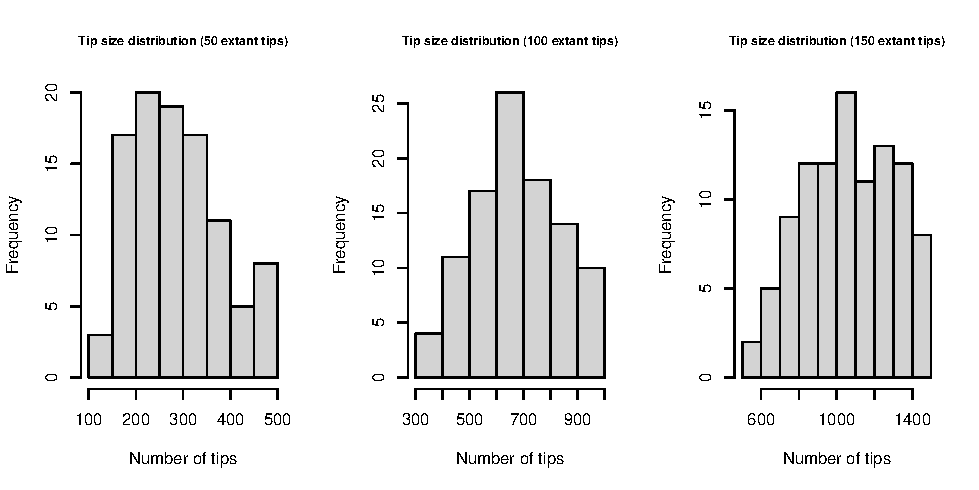
\includegraphics[width=\textwidth]{figures/tree_size_hist.pdf}
\caption{\textbf{Distribution of simulated tree sizes.} Histograms show the final number of extant tips across the three targeted size regimes (50, 100, and 150 extant taxa). Minor variations around the target sizes reflect the stochastic nature of the birth-death simulation process.}
\label{fig:tree sizes} 
\end{figure}


% supplementary
\begin{figure}[H]
\centering
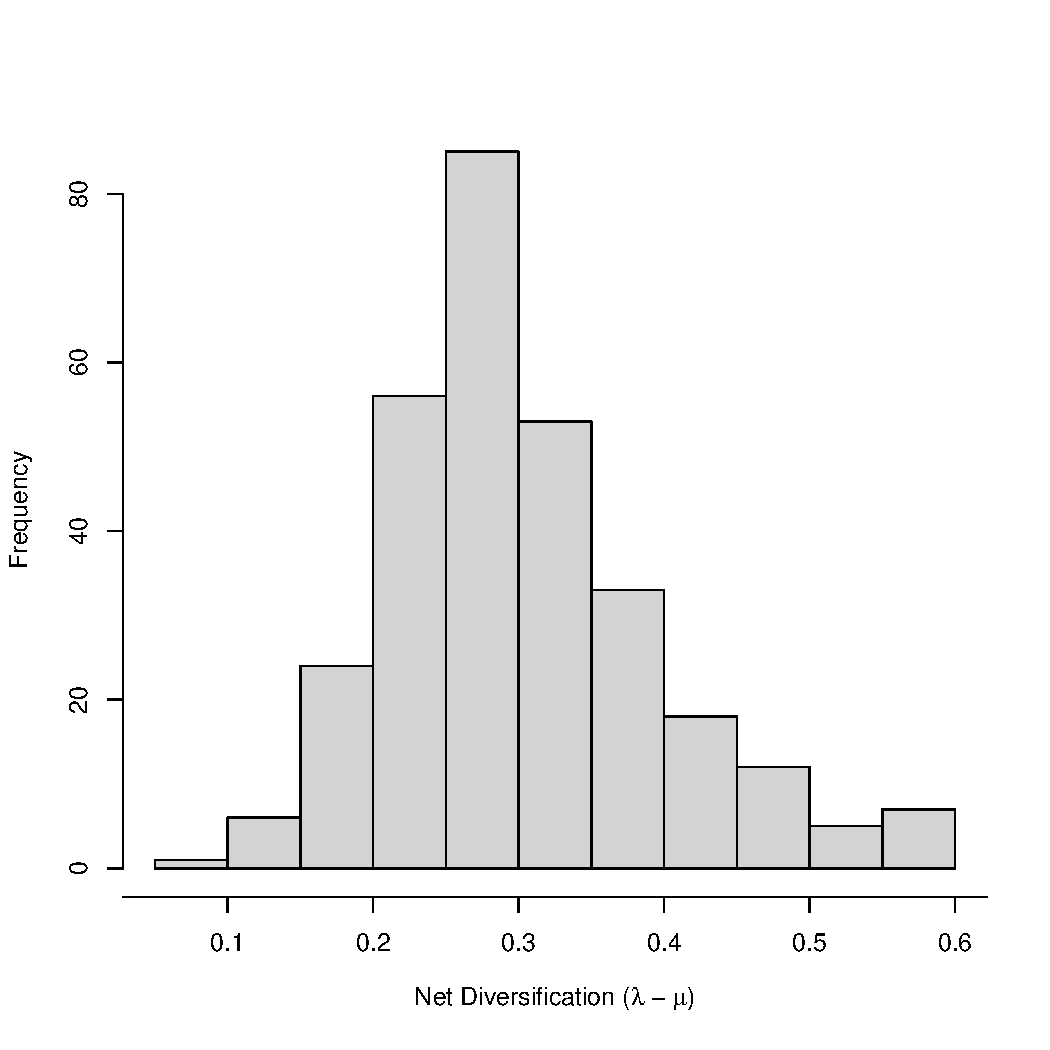
\includegraphics[width=\textwidth]{figures/net_div_hist_overall_trees.pdf}
\caption{\textbf{Birth-death parameters for tree simulation.} The distribution of net diversification (speciation minus extinction) values across all simulated phylogenies.}
\label{fig:net div overall trees} 
\end{figure}


\begin{figure}[H]
\centering
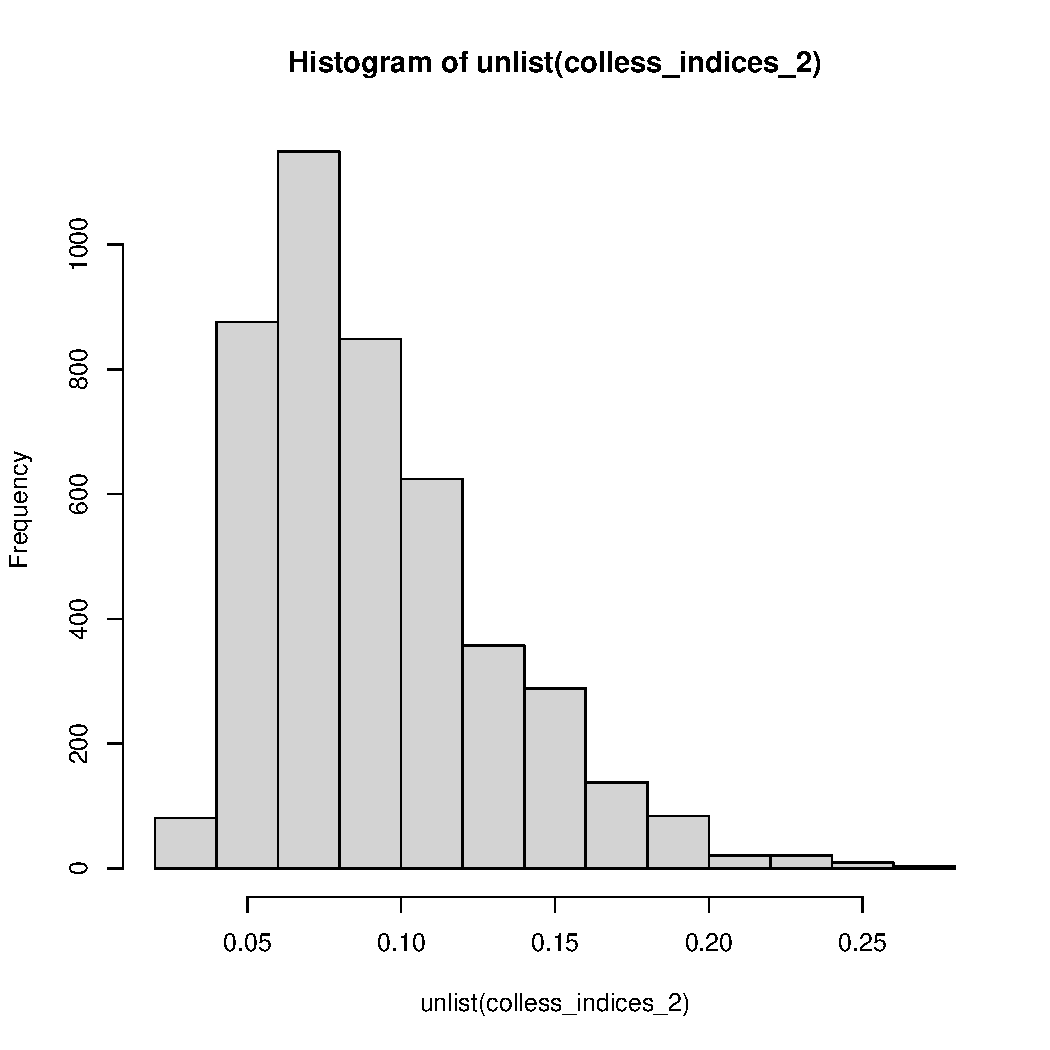
\includegraphics[width =\textwidth]{figures/symmetry.pdf}
\caption{\textbf{Tree symmetry distributions.} Distribution of tree symmetry values measured using the corrected Colless index \citep{heard1992patterns}.}
\label{fig:tree symmetry} 
\end{figure}



\begin{figure}[H]
  \centering
  \includegraphics[width=\textwidth]{figures/aggregated_continuous_diagnostic_plot.pdf}
  \caption{\textbf{Diagnostic plots for the continuous trait linear mixed-effects model (aggregated)}.}
  \label{fig:cont lmm diagnostic aggregated}

\end{figure}


% something wrong here
% \begin{figure}[H]
%   \centering
%   \includegraphics[width=\textwidth]{figures/weighted_continuous_diagnostic_plot.pdf}
%   \caption{\textbf{Diagnostic plots for the continuous trait linear mixed-effects model (weighted)}} \textit{Note:} The diagonal boundary in the Residuals vs fitted plot
%   \label{fig:cont lmm diagnostic aggregated}

% \end{figure}

\begin{figure}[H]
  \centering
  \includegraphics[width=\textwidth]{figures/discrete_diagnostics_aggregated.pdf}
  \caption{\textbf{Diagnostic plots for the discrete trait linear mixed-effects model (aggregated)}} 
  \label{fig:discrete lmm diagnostic aggregated}

\end{figure}

% \begin{figure}[H]
%   \centering
%   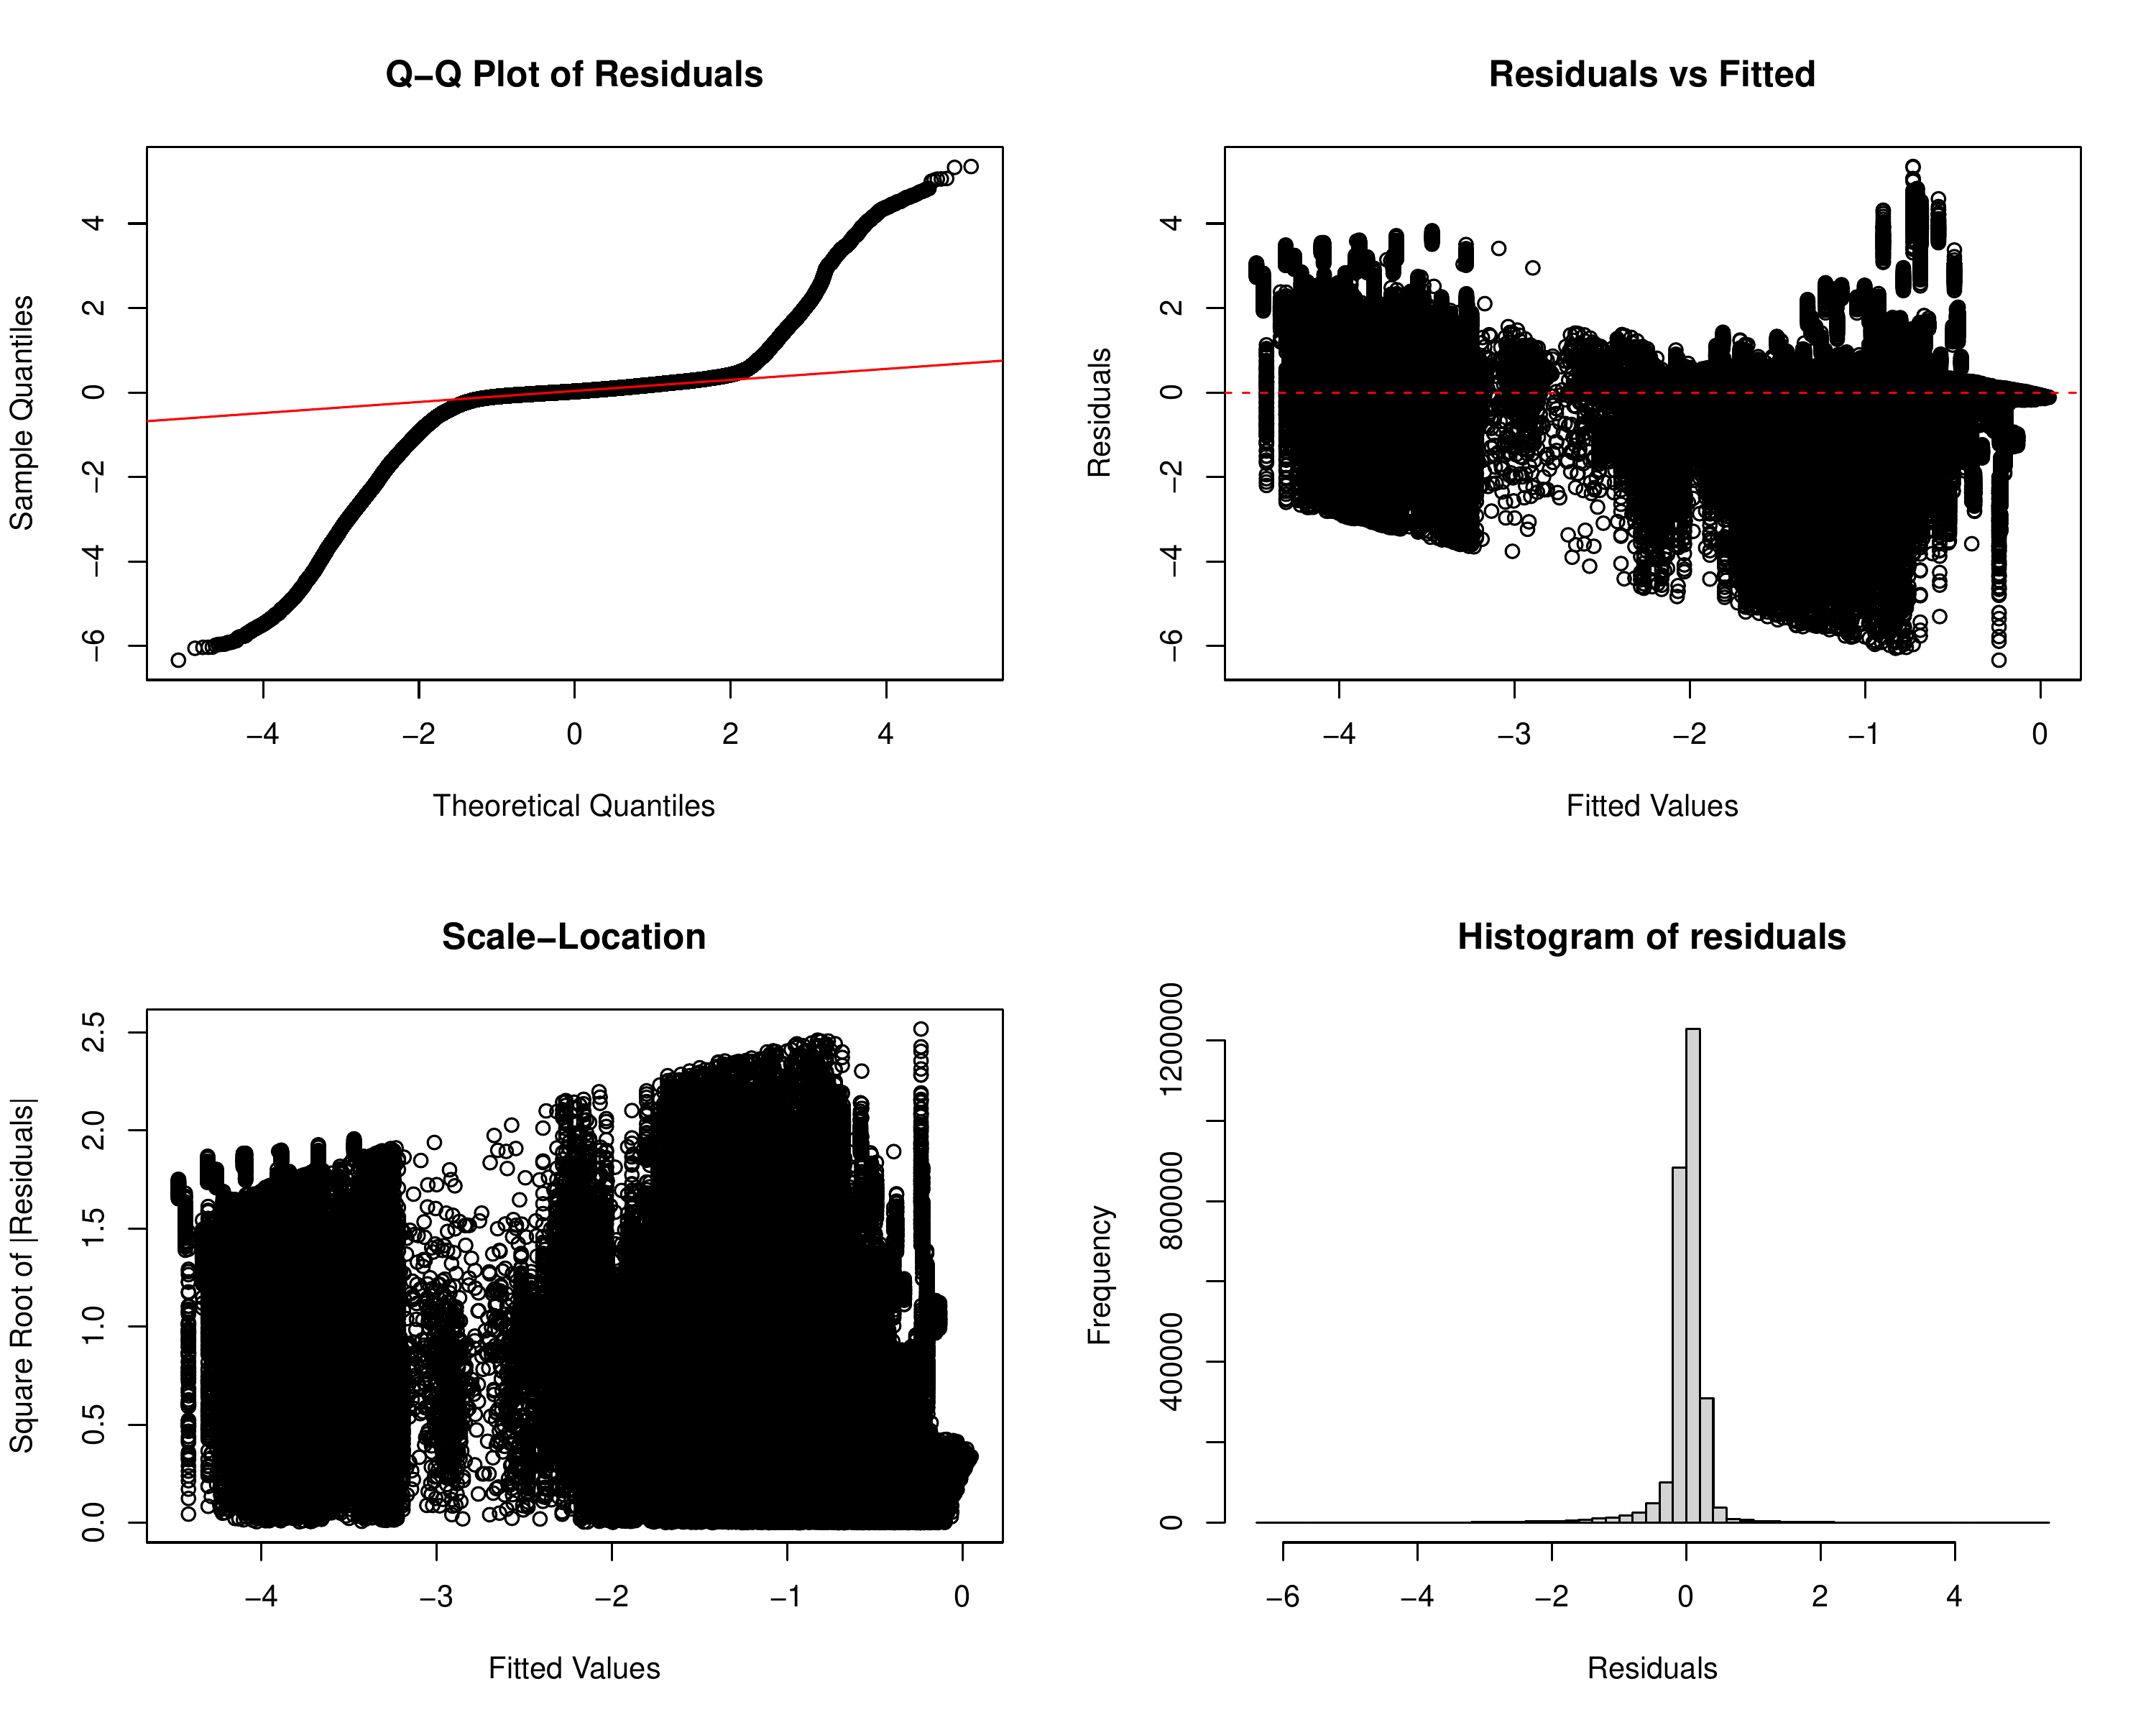
\includegraphics[width=\textwidth]{figures/weighted_discrete_diagnostics.png}
%   \caption{\textbf{Diagnostic plots for the discrete trait linear mixed-effects model (weighted)}} 
%   \label{fig:cont lmm diagnostic aggregated}
% \end{figure}


\begin{figure}[H]
  \centering
  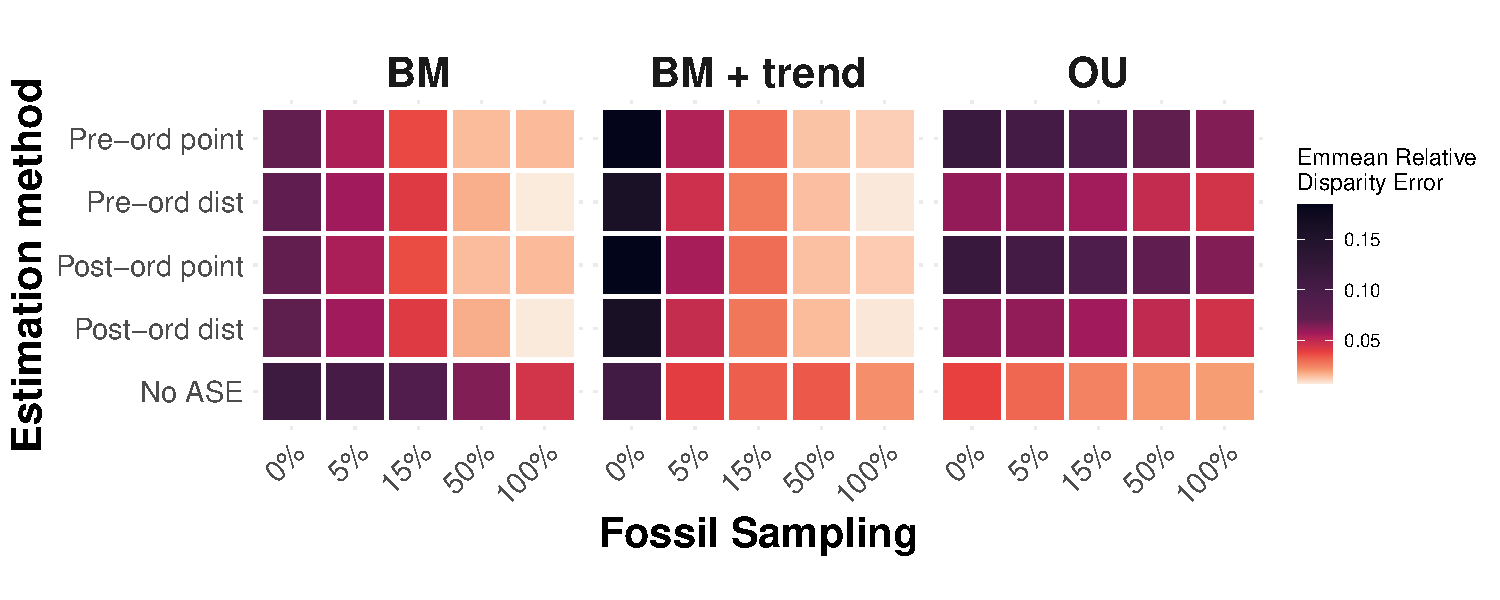
\includegraphics[width=\textwidth]{figures/cont_heatmap_weighted.pdf}
  \caption{\textbf{Weighted LMM continuous heatmap}} 
  \label{fig:weighted LMM continuous heatmap}

\end{figure}



\begin{figure}[H]
  \centering
  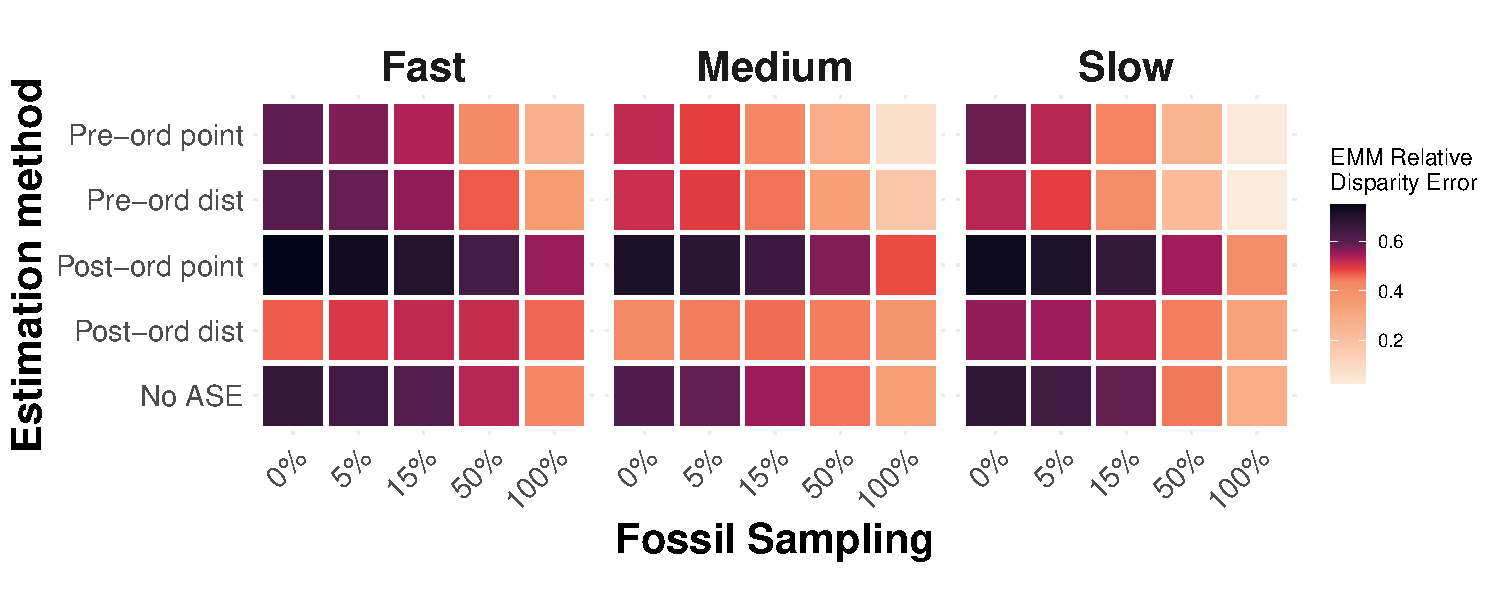
\includegraphics[width=\textwidth]{figures/discrete_weighted_heatmap.pdf}
  \caption{\textbf{Weighted LMM discrete heatmap}} 
  \label{fig:weighted LMM discrete heatmap}
\end{figure}

\bibliographystyle{plainnat}
\bibliography{references.bib}



\end{document}